\documentclass[11pt, a4paper]{article} %twoside
\usepackage{wrapfig}

\usepackage{epigraph}
\usepackage{graphicx}
\usepackage[swedish]{babel}

\usepackage[margin=3cm]{geometry}
\usepackage{float, blindtext, kantlipsum}
%\usepackage{multicol}

\usepackage[toc,page]{appendix}
\usepackage[section=subsection, toc]{glossaries}
\renewcommand{\appendixtocname}{Bilagor} \renewcommand{\appendixpagename}{Bilagor}
\addto\captionsswedish{\renewcommand\appendixname{Bilagor}}


\usepackage[citestyle=verbose-ibid, bibstyle=authoryear, natbib=true, url=false, doi=false, isbn=false, backend=biber, labeldateparts]{biblatex}
\AtEveryBibitem{%
  \clearlist{language}%
  \clearfield{note}%
}
%\usepackage{hyperref}
\addbibresource{bibtex/kandidatarbete.bib}

\usepackage{csquotes}

\usepackage{sectsty}
\subsubsectionfont{\normalfont\itshape}
%\subsectionfont{\normalfont\centering}

\usepackage{titlesec}
\titleformat{\section}
  {\normalfont\LARGE\bfseries}{\thesection}{1em}{}[{}]

  \newcommand{\sectionbreak}{\clearpage}
  %\titlerule[0.8pt]

\makeglossaries
\setglossarystyle{long}

\newglossaryentry{frontend}
{
    name=Front end,
	description={Användargränssnittet i webbutveckling.}
}

\newglossaryentry{backend}
{
    name=Back end,
	description={Allt som rör sig ''under huven'', server-side programmering.}
}

\newglossaryentry{supercollider}
{
    name=SuperCollider,
	description={Ett programmeringsspråk och plattform för syntes av ljud, och musikalisk programmering.}
}

\newglossaryentry{pattern}
{
    name=Pattern,
	description={Ett verktyg i SuperCollider för att generera ...}
}

\newglossaryentry{stack}
{
    name=Stack,
	description={Alla delar som utgör en plattform eller ett system. Finns olika vanligt använda}
}

\newglossaryentry{audification}
{
    name=Audification,
	description={Att direktöversätta en dataserie till ljudkurvor}
}

\newglossaryentry{fifo}
{
    name=FIFO-system,
	description={First in, First out. En typ av kösystem}
}

\newglossaryentry{sonification}
{
    name=Sonifiering,
	description={en. \emph{sonification}. Att översätta en dataserie}
}

\newglossaryentry{mappning}
{
    name=Mappning,
	description={en. \emph{mapping}. Ihopkopplingen av ett datavärde till en parameter. Olika typer av mappningar finns, till exempel \emph{one-to-one} och \emph{one-to-many}}
}

\begin{document}

\tableofcontents
\clearpage


\newpage
%\begin{multicols}{2}

\section*{Introduktion}
\addcontentsline{toc}{section}{Introduktion}
Denna text kompletterar mitt examensprojekt, \emph{Radio Diabetes}, en interaktiv komposition/installation som generarar musik av blodsockervärden. Installationen består av ett SuperCollider-program som skapar själva musiken och en webbplats där man kan lyssna på den, läsa om projektet och ladda upp sina egna blodsockervärden. När en deltagare laddar upp sina värden slussas dessa direkt vidare till SuperCollider-programmet, som i sin tur inkluderar dem i musiken, antingen direkt eller att de blir schemalagda i en kö. Musiken strömmas till webbplatsen (och vidare till lyssnaren) via en internetradiostation. På så sätt utgör musiken ett kontinuerligt flöde som deltagare och åhörare hör samtidigt: det finns ingen början, mitten eller slut, utan endast ett \emph{nu}. %Denna förhållning till \emph{temporalitet} utgör ett huvudtema i projektet, jämte med \emph{interaktivitet} (deltagande), \emph{radioteknologi}, \emph{autoimmuna sjukdomar} och \emph{sonifiering}.

% TODO minska antalet "huvudteman"...?!
% TODO "tystnad i radio"
%\emph{(I skrivande stund är installationen inte helt färdig.)}


\subsection*{Bakgrund}
\addcontentsline{toc}{subsection}{Bakgrund}
Idéen om att göra musik av blodsockervärden föddes dagen då jag fick en \emph{Freestyle Libre}-mätare, en så kallad kontinuerlig blodsockermätare (en. \emph{continous glucose monitoring}, eller \emph{CGM}). Denna typ av blodsockermätare skiljer sig från tradionella mätare --- som man är tvungen att sticka sig i fingret och på så sätt mäta blodsockret med --- i att den regelbundet gör mätningar, vilket ger en kontinuerlig kurva över ens blodsockervärden. Kurvorna påminde mig om hur ljudsignaler ofta representeras visuellt (en horisontell tidsaxel och en linjär vertikal axel) och i ett tidigt experiment gjorde jag en direkt översättning av mina blodsockerkurvor till ljudfiler: en så kallad \emph{audifiering} (en. \emph{audification}). Dessa ljud använde jag som samplingar i mitt stycke \emph{Värden och en vagga} (2017), som var ett av arbetsproverna jag sökte till Musikhögskolan med. 

Jag utvecklade vidare och förbättrade mitt första program som jag hade skrivit för att översätta mina kurvor till ljudfiler, så att vem som helst skulle kunna använda programmet och översätta sina enga värden till ljud. Jag byggde också en wavetable-synth i SuperCollider som använde dessa ljudfiler som källmaterial. Detta instrument har jag använt i ett antal olika kompositioner som jag skrivit under min skoltid. Båda dessa program (översättaren och wavetable-synthen) har jag publicerat på min Github\footcite{jondell_kj-jondelldiabetes-synth_2021}. En del av denna kod återanvände jag även i detta projekt.

\subsection*{Några tidigare exempel, historiska och nutida}
\addcontentsline{toc}{subsection}{Några tidigare exempel, historiska och nutida}
Här har jag valt ut tre exempel ...

Det konstnärliga användandet av biologiska singaler och data har en historia som sträcker sig åtminstone till Alvin Luciers experiment med att komponera musik av hjärnvågor, \emph·{Music for Solo Performer}\footcite{straebel_alvin_2014} från 1965. I detta verk använder Lucier elektroder kopplade till interpretens huvud för att sonifiera dennes alfavågor. De sonifierade hjärnvågorna förstärks och spelas upp i 16 högtalare, som i sin tur exiterar diverse slagverk. I ett seminarium 2001 ska Lucier ha sagt: 

\begin{quote}
  I thought, 'I don't have a structure for this.' I mean, I'm a composer. I should impose some kind of structure, but then I thought, no, brain waves are a natural phenomen. They should just flow out ... %ska jag ha detta som ett block-citat?
\end{quote}


% \usepackage{epigraph}
% \epigraph{}{(B.Parmegiani) \cite{editionsmego}}
% Protein music, DNA music...

%Interaktivitet (\emph{Calling out of context})...

%Radio (\emph{Tuning a radio}, etc...)
\subsection*{Radio}
\addcontentsline{toc}{subsection}{Radio}
En del av installationen består av en internetradiostation, som strömmar ut den genererade musiken. Just denna ...

Radion som konstmedium har länge inspirerat mig, från hörspelen av bland andra Öyvind Fahlström, till John Cages radiokompositioner, till mer sentida \emph{radioqualia}... 

Hot/cool media (McLuhan), interaktion, 

''Ring så spelar vi'' och ''Ring P1'' är två exempel på interaktiva radioprogram, där lyssnarna till hög grad styr och påverkar programmets innehåll. I "Ring P1", som sänds live, är interaktionen så hög att diskussioner kan uppstå lyssnare emellan, där en lyssnare replikerar en annan lyssnares inlägg eller deltagande. Men trots denna höga grad av fri interaktion behöver varje deltagare först passera en telefonsluss. 

%Digital mediekonst som bygger kring internetradio, eller så kallad \emph{streaming culture}, 
%använder sonifieringar

% \emph{r a d i o q u a l i a}...
\subsection*{Sonifiering}
\addcontentsline{toc}{subsection}{Sonifiering}

\gls{sonification}


Sonifiering (eller är det verkligen sonifiering). %\footcite[2]{bijsterveld_sonic_2019}
%Smalley och spektromorfologin. \footnote{Olika ordningar av \emph{surrogacy},  gestaltandet av \emph{datan}.} Bearbetad data och orginaldata. Sensorfel.

\gls{mappning}

\gls{audification} \footcite[302]{noauthor_sonification_2011} är en form av sonifiering där mätdatan översätts direkt till ljudkurvor... fyra grupper av data (\emph{sound recording}, \emph{general acoustic}, \emph{physical}, och \textbf{\emph{abstract}})...

\subsection*{Diabetes}
\addcontentsline{toc}{subsection}{Diabetes}

\subsubsection*{Blodsockervärden}
\addcontentsline{toc}{subsubsection}{\textit{Blodsockervärden}}
Blodsocker mäts i mmol/L och varierar hos en icke-diabetiker mellan 4 och 6 mmol/L [källa]. Hos en diabetiker kan detta värde variera från under 1 till över 30 mmol/L, och Freestyle Libre-sensorn har ett spann på att mäta från lägst 2,2 till 27,7 mmol/L (annars visar den \emph{LO} respektive \emph{HI}). Freestyle Libre-sensorn mäter kontinuerligt var 15:e minut.

%Att s.k. \emph{mappa} denna data till musikaliska parametrar är förstås godtyckligt --- värdena i sig har ingen musikalisk mening --- och bör så vara: det är helt enkelt mina konstnärliga val som bestämmer hur de förhåller sig till varandra. Även en bearbetad signal går att använda för att styra musiken: interpolation (mellan de diskreta mätpunkterna), variation (FFT, derivator, etc.), stokastiska egenskaper (auto-korrelation etc), statistiska egenskaper (median, medel, etc.). ''\emph{Tid i målområdet}'' och liknande värden kan också vara intressanta att använda, och har medicinsk betydelse.

%Det som är viktigt i denna \emph{mappning} är dock att den gestaltade datan --- dvs. musiken --- \textbf{inte} får avslöja något om den underliggande eller bakomliggande (mät)datan. Dels är det en integritetsfråga, som diskuteras vidare nedan, dels är det en förutsättning för detta projekt: det existerar inga \emph{bra} eller \emph{dåliga} värden. Själva delningen av värdena är det viktiga.

\subsubsection*{Förhållandet till mätandet}
\addcontentsline{toc}{subsubsection}{\textit{Förhållandet till mätandet}}
I sin text \emph{Det autoimmuna jaget --- om att sätta gränser} \footcite[286]{arvidson_det_2016} skriver Mats Arvidson om kravet som diabetiker på disciplin \emph{och} prestation.

Prestation, utmattning (bornemark...utmattning...)? Krav och värden... 

Ett sentiment som ofta förekommande (''jag är \textbf{inte} min diabetes, mina blodsockervärden...'', t.ex. artikel i \emph{Hälsoportalen}(???))

\subsection*{Datainsamling}
\addcontentsline{toc}{subsection}{Datainsamling}
Eftersom detta projekt beror av insamling av biometrisk data, som enligt \emph{Dataskyddsförordningen} (GDPR) \footcite{integritetsskyddsmyndigheten_kansliga_nodate} är en känslig personuppgift, krävs ett uttryckligt samtycke från varje deltagare att denna är införstådd i hur datan behandlas. Jag har försökt vara så transparent som möjligt i hur datan behandlas, genom att dels dela \textbf{all} källkod som jag använder, och även i den kommunikation jag lagt ut på webbplatsen och i övriga dokument berörande projektet (såsom denna text). All data som samlas in anonymiseras/avidentifieras så fort som möjligt och den är inte sparad någonstans utöver arbetsminnet som SuperCollider använder. I enlighet med ''God forskningssed'' \footnote{lägg till referens} är anonymitet och integritet av största vikt i detta projekt, även fast det är ett konstprojekt och inte ett forskningsprojekt. Jag har inget kommersiellt intresse i insamlingen av datan, jag delar den inte med någon extern part heller, och allt deltagande är valfritt. Min ambition är \textbf{inte} att samla data för sakens skull, utan att diabetiker ska kunna dela med sig av sina värden utan att de på något sätt bedöms eller värderas: helt enkelt, att själva delandet och deltagandet i sig står i fokus. 

\section*{Process}
\addcontentsline{toc}{section}{Process}
Installationen består som tidigare nämnt av två delar: ett musikgenererande program (SuperCollider) och en webbplats (se figur \ref{hemsida} på nästa sida). Här nedan följer en teknisk beskrivning av detta system.

%\begin{wrapfigure}{l}{0.25\textwidth}
%  \begin{center}
%	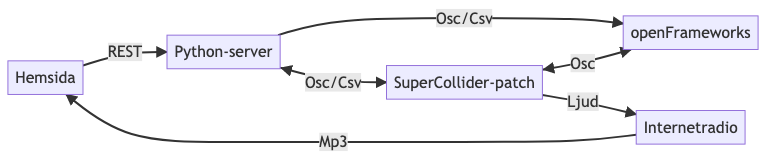
\includegraphics[width=0.23\textwidth]{../media/flowchart.png}
%  \end{center}
%  \caption{Översiktsdiagram av system}
%\end{wrapfigure}

\begin{figure}[H]
\centering
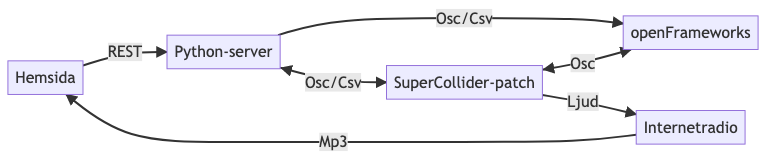
\includegraphics[width=\textwidth]{../media/flowchart.png}
\caption{Översiktsdiagram av system}
\end{figure}

\subsection*{SuperCollider-system}
\addcontentsline{toc}{subsection}{SuperCollider-system}
% TODO LÄGG TILL ETT BLOCKDIAGRAM SOM ILLUSTRERAR SUPERCOLLIDER SYSTEMET
När en deltagare laddar upp en fil med sina mätvärden så skickas de vidare, via Python-servern, till \gls{supercollider}-programmet, som spelar upp en tack-hälsning för att ge en direkt återkoppling till deltagandet. Varje instans av mätdata --- det vill säga varje bidrag till, eller varje interaktion med, installationen --- gestaltas av en specifik musikalisk funktion, för att på sätt ge deltagaren en koppling och förståelse till hur dennes bidrag påverkar musiken. Till exempel kan ett uppladdat paket av data ge upphov till ett arpeggio, någon form av melodi eller en underliggande ljudmatta. I SuperCollider-programmet representeras varje sådan instans av mätdata av ett \emph{objekt}, som innehåller attribut som bland annat: register, skala, speltid, panorering, klangkälla/\emph{SynthDef}, och tillhörande \emph{\gls{pattern}}. Dessa attribut är antingen direkt bestämda av mätdatan (en så kallad \emph{mappning}) eller bestämda utifrån de andra aktiva objekten, till exempel förhåller de sig till redan ''upptagna'' register. Skapandet av dessa objekt gör programmet så fort det mottagit ett nytt paket av mätdata från Python-servern. Samtidigt avgör programmet om objektet ska spelas upp direkt, eller om det ska läggas på kö. 

\subsubsection*{Kösystemet}
\addcontentsline{toc}{subsubsection}{\emph{Kösystemet}}
Behovet av ett kösystem kommer ur scenariot att flera deltagare laddar upp värden inom en relativt kort tidsram. Om detta händer \emph{utan ett kösystem}, kan systemet reagera på två sätt: antingen spelas alla objekt upp samtidigt, med risk för att överrösta varandra och bli en kakofoni, eller så ersätter de varandra, vilket skulle leda till att ens bidrag inte skulle höras mer än en väldigt kort stund. En kompromiss är att använda ett kösystem, så att antalet samtidigt spelande objekt begränsas, och att dessa spelas \emph{minst} en given längd tid, men inte längre än en annan bestämd tid, om det står väntande deltagare på kö. Allt som allt har jag begränsat antalet samtidigt spelande objekt till \emph{tre} stycken, och när dessa är fyllda ställs antingen ett nytt bidrag på kö --- om inte de spelande objekten har varit aktiva i den givna minimumtiden --- eller så ersätter det nya bidraget det äldsta spelande objektet. Kösystemet är i tekniska termer alltså ett \gls{fifo}.

\begin{figure*}[ht!]
\centering
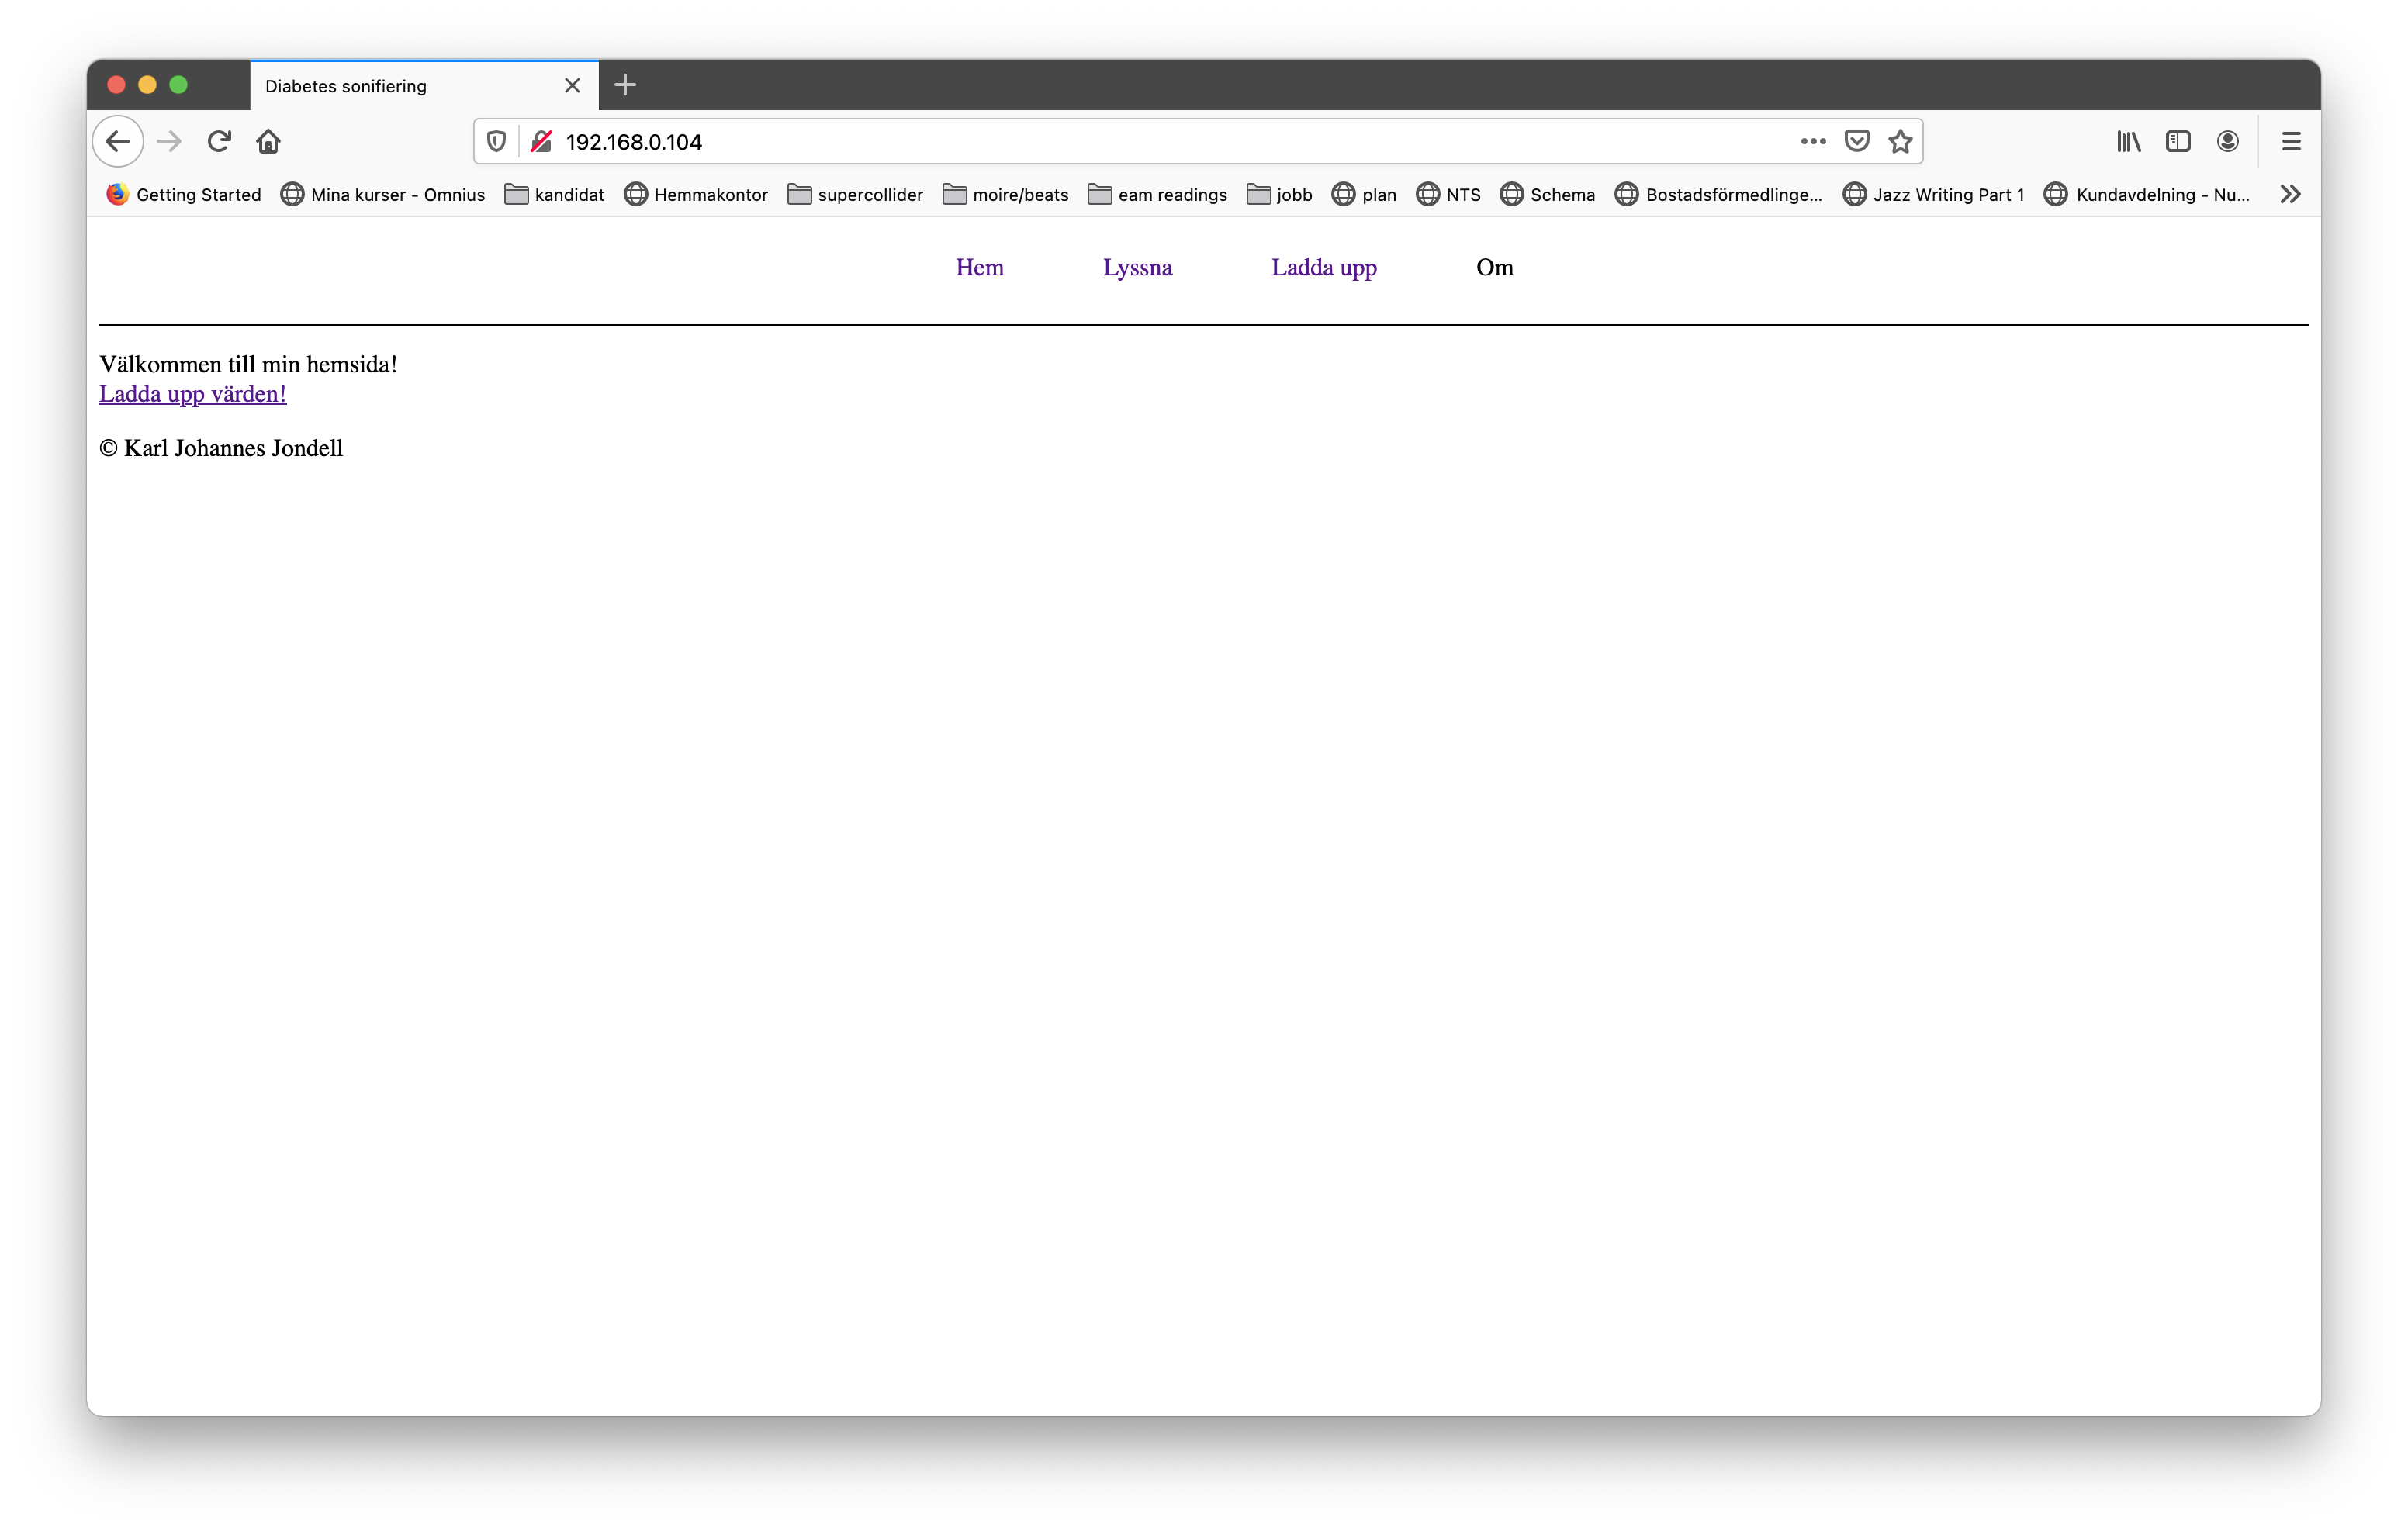
\includegraphics[width=\textwidth]{../media/hemsida.png}
\caption{Skärmdump av hemsida (\emph{temporär})}
\label{hemsida}
\end{figure*}

\subsection*{Webbplats}
\addcontentsline{toc}{subsection}{Webbplats}

Webbplatsen finns i skrivande stund tillgänglig på domänen: \url{https://radiodiabetes.eu/}\footcite{jondell_radio_nodate}. I figur \ref{hemsida} på föregående sida visas en skärmdump av webbplatsen tagen den... %TODO insert date....

Webbplats består av en s.k. \emph{\gls{frontend}} och en \emph{\gls{backend}}. Linux (Ubuntu 20.04)/Nginx/gunicorn \gls{stack}.
\subsubsection*{Front end}
\addcontentsline{toc}{subsubsection}{\emph{Front end}}
1. beskriv vad frontend är för något
2. beskriv tekniken (react.js)

\subsubsection*{Back end}
\addcontentsline{toc}{subsubsection}{\emph{Back end}}
1. beskriv vad backend är för något (API?)
2. flask, darkice/icecast också kanske? 

\subsection*{Tillvägagångssätt}
\addcontentsline{toc}{subsection}{Tillvägagångssätt}
Hur jag gjort/reflektioner/vad jag ändrat

\section*{Musiken}
\addcontentsline{toc}{section}{Musiken}


% Lager, eller vilka SynthDefar jag har:
% 1. GSM (drone, eller bas/fundament, eller pad...)
% 2. Sinusvågor och elektroniska störningsljud (arpeggio, rytmiska, sextondelar, tempo)
% 3. Wavetable (pad)
% 4. JLC bas? resonator hum ? andra ljud ? ?? ? ? 

De musikaliska funktioner jag har representerade är dels ett fundament eller grund som utgörs av ett 

%Den konstnärliga friheten. Hur pass mycket kontroll som överlåtes till \enquote{serien} (i detta fall blodsockervärdet). Behöver musiken gestalta, spegla, estetisera erfarenheten som diabetiker? Eller vara intresseväckande, tillgänglig, \enquote{relaterbar}? 

\subsection*{Rumslighet}
\addcontentsline{toc}{subsection}{Rumslighet}
Varje objekt ges en unik position i stereofältet, och på så sätt en plats i rummet i musiken. 

Presentationen av radioströmmen genom hemsidan som jag har utformat påverkar också den upplevda rumsligheten i musiken. 

Ett planerat konserttillfälle kommer att ske den 20e maj i Lilla Salen i Musikhögskolan. Då spelas ett utdrag ur radioströmmen upp, som den hörs i realtid. I och med de rådande restriktionerna så kommer ingen publik kunna närvara, utan konserten strömmas vidare till en publik i etern. Själva konserttillfället blir därför en sorts manifestation av radioströmmen i tid och rum. 


% TODO tempusformulering


\subsection*{Temporalitet}
\addcontentsline{toc}{subsection}{Temporalitet}
Den tidsmässiga uppfattningen av musiken. En 24/7 livestream av musiken (hur utgörs lyssnadet? formen? \emph{Slow as possible}, \emph{Longplayer} och liknande...)

\subsection*{Generativt}
\addcontentsline{toc}{subsection}{Generativt}
Musiken är generativ. Serialism?

\section*{Slutsatser}
\addcontentsline{toc}{section}{Slutsatser}
Lärdomar etc...

\subsection*{Utvecklingsmöjligheter}
\addcontentsline{toc}{subsection}{Utvecklingsmöjligheter}
För mig är detta endast startskottet på ett projekt som kan växa på alla sätt. Jag har byggt en infrastruktur till en installation som går att utveckla.

- Gästbok/lämna röstmeddelanden...
- Två strömmmar: kunna växla mellan dem för att möjliggöra enklare utveckling av SuperCollider-systemet (utan att det behöver stängas ned för underhåll).
- Möjligheten att spela upp binauralt
- Internationellaisera (översätt hemsida etc...)

%\end{multicols}


%\twocolumn
%\clearpage
\addcontentsline{toc}{section}{Referenser}
\printbibheading
\printbibliography[type=book,title={Böcker},heading=subbibliography]
\printbibliography[type=article,title={Artiklar},heading=subbibliography]
\printbibliography[type=online,title={Hemsidor},heading=subbibliography]

\clearpage
\begin{appendices}
\printglossary[nonumberlist]
\end{appendices}

\end{document}

